\chapter{Prime Power ORC System Model}
\label{ch:model}

The model attempts to recreate a microgrid which uses an ORC fed by geothermal resources as a primary power source in order to form a grid with a self-excited induction generator using full power electronic conversion. \autoref{fig:full_flow_diagram_label} shows the ORC prime power system model flow diagram with all the variable inputs on the left and outputs on the right. The internal blocks include the ORC, the pump drive motor, the SEIG, and the full power electronic grid-forming inverter. The ORC block, itself, is composed of evaporating and condensing heat exchangers, as well as a pump and expander, both of which are assumed to be non-ideal isentropic processes.
\begin{figure}[h]
	\centering

	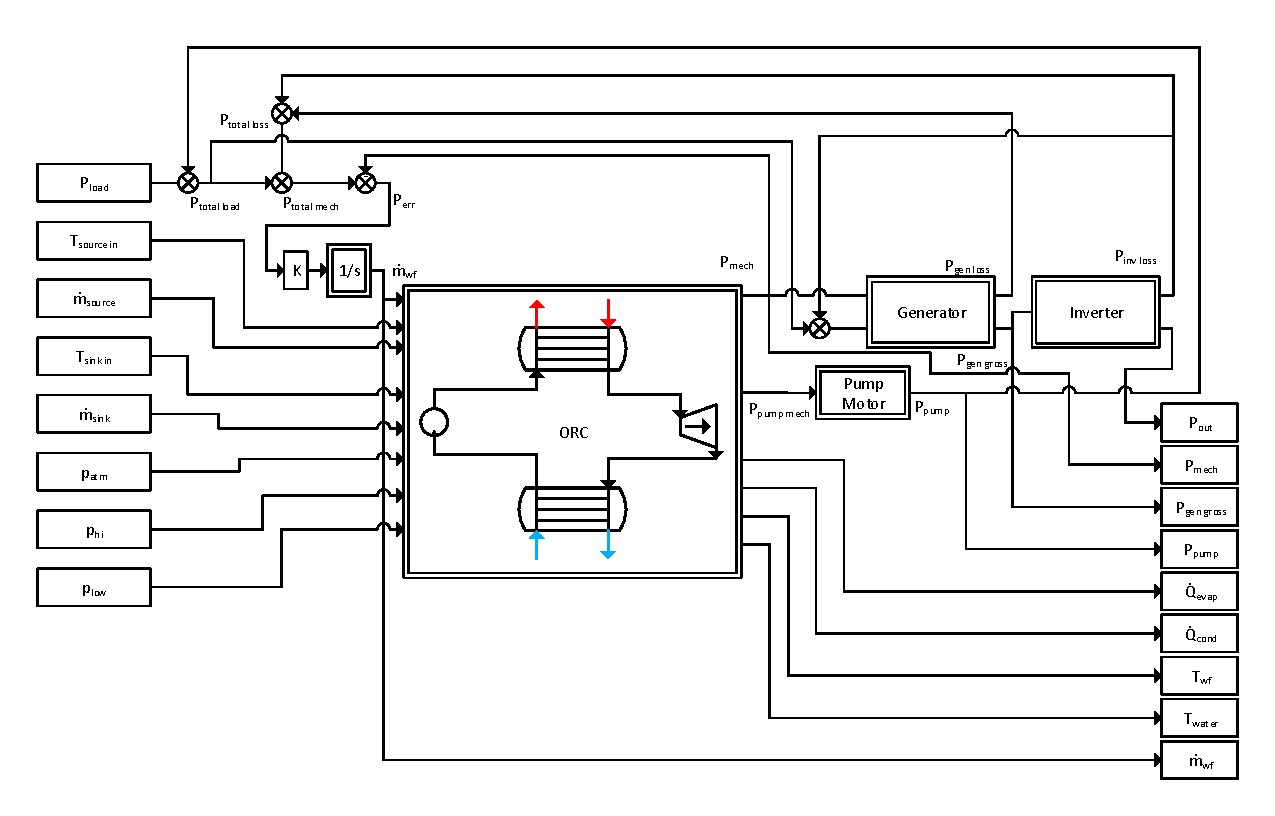
\includegraphics[width=\textwidth]{figures/Full Model Flow Diagram.pdf} 

	\caption{Organic Rankine cycle prime power system model diagram documenting data flows of the model. Boxes on the left side represent variable inputs, and those on the right indicate variable outputs.}
	\label{fig:full_flow_diagram_label}

\end{figure}

\section{Organic Rankine Cycle}
The ORC block, seen in \autoref{fig:orcblock_label} links the thermal, mechanical, and electrical components of the model. The thermal properties of the source, sink, and working fluids were obtained from a MATLAB\textsuperscript{\textregistered} wrapper of the CoolProp\textsuperscript{\textcopyright} library. Thermal conditions of source, sink, and working fluids are input to the Rankine cycle portion of the model which returns a mechanical power. 
%Electrical conditions, along with the mechanical power, are input in the generator portion of the model which returns an electrical output. 
\input{figures/orcblock}

CoolProp\textsuperscript{\textcopyright} is an open source C++ library which contains thermophysical properties of over 110 fluids including the working fluids used in refrigeration processes \cite{Bell2014}. It makes use of Helmholtz energy-explicit equations of state to derive its values, but can also incorporate the REFPROP library developed by the National Institute of Standards and Technology (NIST). Although originally written for C++, wrappers have been developed for many other common programming languages and analytical software including, but not limited to, MATLAB\textsuperscript{\textregistered}, Python, Java, R, NI Lab View\textsuperscript{\texttrademark}, and Excel. Due to its wide availability and open source licensing, it has seen much use in the analysis of ORCs \cite{Pezzuolo2016, Pierobon2014}, refrigeration units \cite{Besagni2015}, and other applications \cite{Quoilin2014, Nilsen2016}.
\nomenclature[B]{NIST}{National Institue of Standards and Technology}

In order to use CoolProp\textsuperscript{\textcopyright}, first a handle is initialized for each of the source, sink, and working fluids. The handle is passed as a static parameter to any of the functions that require any thermophysical calculations. The function uses the handle during any calls of the CoolProp\textsuperscript{\textcopyright} library.

The variable inputs used for the ORC block include the mass flow rates for the source, $\dot{m}_{source}$, sink, $\dot{m}_{sink}$, and working fluids, $\dot{m}_{wf}$ (\si{\kilogram\per\second}), the inlet temperature of the source, $T_{source\ in}$, and sink, $T_{sink\ in}$ (\si{\kelvin}), the absolute pressures for the high side, $p_{hi}$, and low side of the cycle, $p_{low}$, as well as the pressures of source, $p_{source\ in}$, and sink fluid inlets, $p_{sink\ in}$ (\si{\pascal}). In these simulations, $p_{source\ in}$ and $p_{sink\ in}$ are both assumed to be at atmospheric pressure, $p_{atm}$, though that is not a necessary condition. Fixed input parameters include the initial mass specific enthalpy of the working fluid feeding into the evaporator, $h_{init}$ (\si{\joule\per\kilogram}), as well as several values described in \autoref{sec:heatex} and \autoref{sec:isentrope}.
\nomenclature[S]{$_{source}$}{Source fluid}
\nomenclature[S]{$_{sink}$}{Sink fluid}
\nomenclature[S]{$_{init}$}{Inital condition of the working fluid}
\nomenclature[S]{$_{hi}$}{High pressure side of the cycle}
\nomenclature[S]{$_{low}$}{Low pressure side of the cycle}
\nomenclature[S]{$_{atm}$}{Atmospheric pressure}

Before the inputs are fed into the sub-blocks, the fluid temperature and pressure combinations are converted to mass specific enthalpy values using CoolProp\textsuperscript{\textcopyright}. Similarly, mass specific enthalpy and pressure combinations are converted to temperatures before being output.

The output variables from the ORC block include the mechanical power produced by the expander, $P_{mech}$ and consumed by the pump, $P_{mech\ pump}$ (\si{\watt}), the heat flow rates of the evaporator, $\dot{Q}_{evap}$, and condenser, $\dot{Q}_{cond}$ (\si{\watt\textsubscript{th}}), and the temperatures of the water, $T_{water}$, and working fluid, $T_{wf}$ (\si{\kelvin}), at various points in the cycle. Specifically, $T_{water}$ is composed of the inlet and outlet temperatures of the source and sink fluids, while $T_{wf}$ contains temperatures at the inlets and outlets of the pump and expander and assumes there is no temperature drop through the lines to and from the heat exchangers.

\subsection{Evaporator and Condenser}
\label{sec:heatex}
The evaporator and the condenser are both represented using a heat exchanger script.  A block diagram of the function can be seen in \autoref{fig:heatexblock_label}. The function takes as inputs variables characterizing hot and cool fluids, specifically the inlet mass specific enthalpies, $h_{h,i}$ and $h_{c,i}$ (\si{\joule\per\kilogram}), mass flow rates, $\dot{m}_{h,i}$ and $\dot{m}_{c,i}$ (\si{\kilogram\per\second}), and inlet pressures, $p_{h,i}$ and $p_{c,i}$ (\si{\pascal}). Additional static inputs include CoolProp\textsuperscript{\textcopyright} fluid handles, as well as parameters characterizing the exchanger itself such as the overall heat transfer coefficient, $U$ (\si{\watt\per\kelvin\per\meter\squared}), the heat transfer area, $A$ (\si{\meter\squared}), and a string describing the heat exchanger type (e.g. counter or parallel flow). The function output is made up of the heat flow rate, $\dot{Q}$ (\si{\watt}\textsubscript{th}), and the mass specific enthalpies at the outlets, $h_{h,o}$ and $h_{c,o}$ (\si{\joule\per\kilogram}). 
\begin{figure}[h]
	\centering

	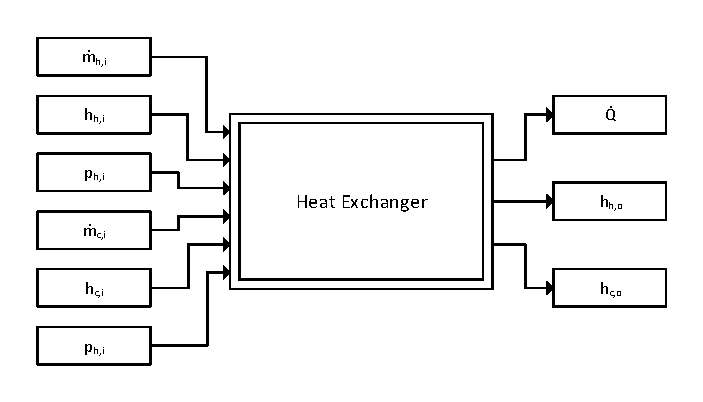
\includegraphics[width=\textwidth]{figures/HeatExBlock.pdf} 

	\caption{Heat exchanger NTU model diagram showing variable inputs on the left and outputs on the right.}
	\label{fig:heatexblock_label}

\end{figure}

In order to calculate the desired values, the Number of Transfer Units (NTU) method is used. Described in The Fundamentals of Heat and Mass Transfer \cite{Incropera}, this process calculates the output heat flow, $\dot{Q}$, relative to a theoretical maximum heat flow, $\dot{Q}_{max}$. This potential heat flow would be realized using an infinitely long counter flow geometry and is calculated as
\begin{equation}
\dot{Q}_{max} = C_{min}\left(T_{h,i} - T_{c,i}\right)
\end{equation}
where $C_{min}$ is the smaller heat capacity rate of the hot and cool fluids and $T_{h,i}$ and $T_{c,i}$ are the inlet temperatures of hot and cool fluids, respectively. The heat capacity rate is the product of mass flow rate, $\dot{m}$, and the mass specific heat at constant pressure, $c_p$, or 
\begin{equation}
C = \dot{m} \cdot c_p. 
\end{equation}
\nomenclature[V]{$\dot{Q}$}{Themal heat flow rate\nomunit{\si{\kilo\watt}\textsubscript{th}}}
\nomenclature[V]{$C$}{Heat capacity rate of a fluid\nomunit{\si{\joule\per\second\per\kelvin}}}
\nomenclature[V]{$NTU$}{Number of transfer units of a heat exchanger\nomunit{\si{\kelvin\second\per\joule}}}
\nomenclature[V]{$\dot{m}$}{Mass flow rate\nomunit{\si{\kilogram\per\second}}}
\nomenclature[V]{$c_p$}{Mass specific heat of a fluid at constant pressure\nomunit{\si{\joule\per\kilogram\per\kelvin}}}
\nomenclature[S]{$_{min}$}{Minimum}
\nomenclature[S]{$_{max}$}{Maximum}
\nomenclature[S]{$_{h,i}$}{Hot fluid inlet}
\nomenclature[S]{$_{c,i}$}{Cool fluid inlet}

The heat flow rates of the hot and cool fluids are related by the effectiveness, $\epsilon$, which is defined as 
\begin{equation}
\label{eq:effectiveness_def}
\epsilon \equiv \frac{\dot{Q}}{\dot{Q}_{max}}.
\end{equation}
\nomenclature[V]{$\epsilon$}{Effectiveness of a heat exchanger.}
Numerically, the value of $\epsilon$ is a function of the ratio of the fluids' heat capacity rates, 
\begin{equation}
C_r = \frac{C_{min}}{C_{max}},
\end{equation}
as well as the exchanger's Number of Transfer Units, 
\begin{equation}
NTU = \frac{U \cdot A}{C_{min}},
\end{equation}
where $U$ is the overall heat transfer coefficient and $A$ is the total heat transfer area. Additionally, the direction of fluid flow changes the method of calculation. In parallel flow heat exchangers the effectiveness is calculated as
\begin{equation}
\epsilon = \frac{1 - \exp\left[-NTU\left(1 + C_r\right)\right]}{1 + C_r}
\end{equation}
while counter flow devices use
\begin{equation}
\epsilon = \frac{1 - \exp\left[-NTU\left(1 - C_r\right)\right]}{1 - C_r\exp\left[-NTU\left(1 - C_r\right)\right]}.
\end{equation}
\nomenclature[V]{$U$}{Overall heat transfer coffecicient of a heat exchanger\nomunit{\si{\joule\per\meter\squared\per\second\per\kelvin}}}
\nomenclature[V]{$A$}{Heat transfer area of a heat exhcanger\nomunit{\si{\meter\squared}}}
\nomenclature[S]{$_{r}$}{Ratio}

Once the effectiveness and maximum heat transfer rate are determined, equation \ref{eq:effectiveness_def} is used to calculate the actual rate of heat flow, $\dot{Q}$. Finally, the change in temperature for each fluid is calculated based on their respective heat capacity rates at initial conditions and the rate of heat flowing between them. 
If the change in temperature for either fluid would result in vaporization or condensation, then the values must be recalculated because the specific heat is effectively infinite while the fluid is changing states. 

First, the heat flow rate necessary to have the fluid begin changing its state is determined and the fraction of this value relative to the initial heat flow rate is calculated. 
The heat transfer area is reduced by this fraction and the function is repeated by inputing the state of the two fluids as the one fluid begins to change phase. If enough heat flows between the two fluids such that the one completes the phase change, then the function is repeated a third time with the heat transfer area modified again. 

Within this script there are certain assumptions made in order to calculate the output values. The function will not return accurate results if both fluids simultaneously undergo a phase change because the ratio of heat capacities, $C_r$, will be undefined. Additionally, ambient temperature and associated heat flow to the external environment is not accounted for in the script. Finally, it is assumed the pressure drop from inlet to outlet is negligible for both the high and low temperature fluids. 
\nomenclature[S]{$_{wf}$}{Working fluid}
\nomenclature[S]{$_{water}$}{Water}

%This process is used for both the evaporator and the condenser. For the evaporator, the 

\subsection{Expander and Pump}
\label{sec:isentrope}
The expander/turbine and pump components are both modeled by a fluid undergoing non-ideal isentropic expansion or compression. For an ideal isentropic process, the fluid will experience some thermodynamic changes while its internal entropy remains constant. During this process, power is produced if the pressure at the inlet is greater than at the outlet, and consumed if inlet pressure is less than that of the outlet. A block diagram of the function can be seen in \autoref{fig:isentropeblock_label}.
\begin{figure}[h]
	\centering

	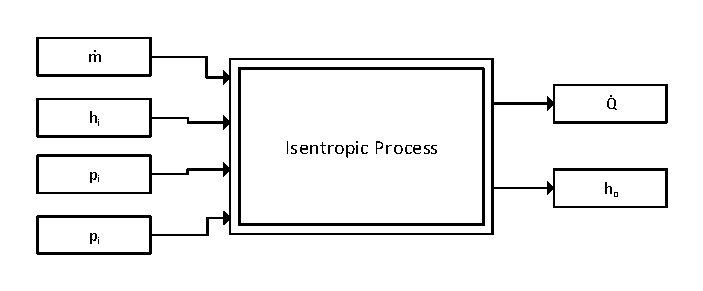
\includegraphics[width=\textwidth]{figures/IsentropeBlock.pdf} 

	\caption{Isentropic model diagram showing variable inputs on the left and outputs on the right.}
	\label{fig:isentropeblock_label}

\end{figure}

The function takes as inputs certain properties of the fluid, such as the inlet mass specific enthalpy, $h_i$ (\si{\joule\per\kilogram}), both the inlet and outlet pressures, $p_i$ and $p_o$ (\si{\pascal}), and the mass flow rate, $\dot{m}$ (\si{\kilogram\per\second}). Also needed is the fluid CoolProp\textsuperscript{\textcopyright} handle and the isentropic efficiency, $\eta$, a unitless parameter of the machine which describes power loss due to deviations from the ideal isentropic process. The function returns the mechanical power produced or consumed, $P$ (\si{\watt}), and the mass specific enthalpy of the fluid at the outlet, $h_o$ (\si{\joule\per\kilogram}).

Using the inputs and the CoolProp\textsuperscript{\textcopyright} library, the mass specific entropy, $S$, of the fluid is determined for the fluid at the inlet. In an ideal process this value would remain constant so here it is used to determine the ideal enthalpy of the outlet. Next the ideal power transferred is calculated as 
\begin{equation}
\label{eq:power_enthalpy}
P = \dot{m} \left(h_i - h_o\right)
\end{equation}
where $h_i$ and $h_o$ are the inlet and outlet mass specific enthalpies, respectively.
\nomenclature[V]{$P$}{Mechanical or active electrical power\nomunit{\si{\kilo\watt}}}
\nomenclature[V]{$S$}{Mass specific entropy of a fluid\nomunit{\si{\joule\per\kilogram\per\kelvin}}}
\nomenclature[S]{$_{i}$}{Inlet}
\nomenclature[S]{$_{o}$}{Outlet}

To obtain the mechanical power actually transferred, the isentropic efficiency is applied to the ideal power such that the ideal power is necessarily greater than the actual power. When the value of $h_i$ is larger than $h_o$, $P$ is positive therefore efficiency is multiplied. When $h_i$ is less than $h_o$, $P$ is negative and ideal power is divided by efficiency. After the mechanical power is calculated, equation \ref{eq:power_enthalpy} is used to find $h_o$ and the fluid temperature at the outlet. 

\section{Induction Generator}
The generator block models a squirrel cage induction generator (SCIG) in order to convert the mechanical power to an electrical form. Furthermore, 
%Two different function blocks were created for two scenarios: regulated and unregulated. The former is simpler to model, but the generator requires another firm source\footnote{Or an electrical storage-inverter combination.} to maintain its frequency and voltage. For the latter scenario, the generator's frequency and voltage are allowed to vary. Its leads are connected directly to a power converter which maintains the frequency and voltage of the microgrid. 
to simulate microgrids with no forms of storage or sources beyond the ORC, it is also self-excited. 
%The single phase equivalent circuit %is similar to the regulated SCIG circuit 
%can be seen in \autoref{fig:SCIG__circuit_diagram}.
%, except the voltage source $V_{ph}$ at the output terminals of the machine is replaced with a resistive load. 
The model is based off the analysis by Ouazenne et al. of a self excited induction generator in \cite{Ouazenne1983} using admittance balancing. It is assumed the active power losses across the core and the excitation capacitance are negligible. Additionally, it is assumed the load is purely active, as any reactive load can be supplied by the conversion device which regulates the frequency and voltage of the microgrid.
\nomenclature[B]{SCIG}{Squirrel cage induction generator}

The method of admittance balancing relies on the fact that active and reactive power entering and exiting an electrical node must sum to zero. For this analysis, the chosen node is where the rotor, the core, and the combination of the stator, excitation capacitor, and load meet and labeled A in \autoref{fig:SCIG__circuit_diagram}. Since the voltage across each branch is the same and power flow sums to zero, the admittances must sum to zero as well. By breaking the complex admittances into real and imaginary components, a system of equations can be developed to solve for frequency and core reactance. 
\begin{figure}[h]
	
\centering

\begin{tikzpicture}[american voltages]
\draw[color=black, thick]
%Input
(0,0) to [open, l=$V_{ph}$, o-o] (0,4){}

%low
(0,0) -- (9,0){}

%stator
(0,4) -- (1.5,4) to [R, l=$R_{s}$] (3,4) to [L, l = $j X_{s}$] (4.5,4){}

%rotor
(4.5,4) -- (5.5,4) to [R, l=$R_{r}$] (7.5,4) to [L, l = $j X_{r}$] (9,4) to [R, l=$R_{r}\frac{1-s}{s}$] (9,0){}

%core
(5,4) to [short, *-*] (5,3){}
(4.5,3) -- (5.5,3) to [L, l = $j X_{m}$] (5.5,1) -- (4.5,1) to [R, l=$R_{c}$] (4.5,3){}
(5,1) to [short, *-*] (5,0){}

%external excitaion capacitor
(1,4) to [R, l=$R_{esr}$, *-] (1,2) to [C, l=$-j X_x$] (1,0.5) to [short, -*] (1,0){}


;
\end{tikzpicture}

\caption{Single phase diagram of a three phase squirrel cage induction machine. $V_{ph}$ and $s$ are the phase voltage and slip of the generator. }
\label{fig:SCIG__circuit_diagram}

\end{figure}

%\subsection{Regulated SCIG}
%This function block takes several electrical and mechanical parameters as inputs such as the line to line voltage (\si{\volt}) and electrical frequency (\si{\hertz}) at the output terminals of the machine, the mechanical speed at the shaft (\si{\rpm}), the number pole pairs in the machine's stator windings, and coefficients of friction due to bearings (\si{\watt\per\second}) and windage (\si{\watt\per\second\squared}). Other inputs are the resistive and inductive impedances (\si{\ohm}) of the stator, rotor, and core, as well as the capacitive impedance and equivalent series resistance of external excitation capacitor. The function returns the active (\si{\watt}) and reactive (\si{\voltampreactive}) power outputs and losses.
The block, seen in \autoref{fig:scigblock_label} takes as variable inputs the mechanical power produced by the shaft, $P_{mech}$ (\si{\watt}), and 
%speed of the shaft (\si{\rpm}), 
the combined power of the total load and the inverter losses, $P_{total\ load} + P_{inv\ loss}$ (\si{\watt}) as seen by the generator. The block outputs include the gross active power produced, $P_{gen\ gross}$ (\si{\watt}), and the active power losses of the generator, $P_{gen\ loss}$ (\si{\watt}).
%, the mechanical power needed to generate the output, $ P_{mech\ needed}$ (\si{\watt}), and the line to line voltage, $ V_{ll}$ (\si{\volt}).
\begin{figure}[h]
	\centering

	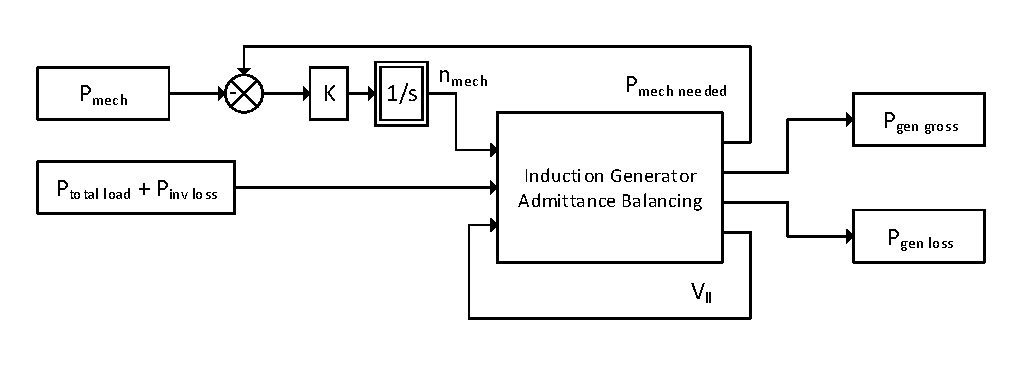
\includegraphics[width=\textwidth]{figures/SCIGBlock.pdf} 

	\caption{Self-excited squirrel cage induction generator model diagram showing variable inputs on the left and outputs on the right.}
	\label{fig:scigblock_label}

\end{figure}
\nomenclature[S]{$_{gen}$}{Generator}
\nomenclature[S]{$_{gross}$}{Gross output}
\nomenclature[S]{$_{loss}$}{Device losses}

To calculate the output variables a function was developed to implement the admittance balancing equations. This function takes the input variables of the rotor speed, $n_{mech}$ (\si{\rpm}), the combined load as seen by the generator, $P_{total\ load} + P_{inv\ loss}$ (\si{\watt}), and the line to line voltage magnitude, $\left|V_{ll}\right|$ (\si{\volt}). The output variables of the function include active power generated, $P_{gen\ gross}$ (\si{\watt}), and internally consumed, $P_{gen\ loss}$ (\si{\watt}), 
%the reactive power consumed (\si{\voltampreactive}), 
the necessary mechanical power driving the shaft, $P_{mech\ needed}$ (\si{\watt}), and the re-calculated line to line voltage magnitude, $\left|V_{ll}\right|$ (\si{\volt}). The value of $n_{mech}$ is determined by comparing $P_{mech}$ and $P_{mech\ needed}$ from the previous time step, then integrated with an appropriate proportionality constant, $K$. This control scheme increases $n_{mech}$ when $P_{mech\ needed}$ is less than $P_{mech}$ and vice versa.
%, and the electrical frequency (\si{\hertz}).
\nomenclature[S]{$_{inv}$}{Inverter}
\nomenclature[S]{$_{mech\ needed}$}{Mechanical power needed}

The fixed parameter inputs to the admittance balancing function block are the rated frequency of the machine, $f_{rated}$ (\si{\hertz}), the number of poles, the resistances (\si{\ohm}) and inductances (\si{\henry}) of the rotor, $R_r$ (\si{\ohm}) and $L_r$ (\si{\henry}), and stator, $R_s$ (\si{\ohm}) and $L_s$ (\si{\henry}), the external excitation capacitors, $C_x$ (\si{\farad}), coefficients of friction due to bearings, $K_{bearing}$ (\si{\watt\per\second}), and windage, $K_{windage}$ (\si{\watt\per\second\squared}), and the magnetization curve comparing the core reactance, $X_m$ (\si{\ohm}) to the internal voltage across the core, $E$ (\si{\volt}). 
\nomenclature[V]{$R$}{Resistance\nomunit{\si{\ohm}}}
\nomenclature[V]{$X$}{Reactance\nomunit{\si{\ohm}}}
\nomenclature[V]{$L$}{Inductance\nomunit{\si{\henry}}}
\nomenclature[V]{$E$}{Internal induced voltage of rotating machine\nomunit{\si{\volt}}}
\nomenclature[V]{$n$}{Rotational velocity\nomunit{\si{\rpm}}}
\nomenclature[V]{$poles$}{Number of poles in electrical machine}
\nomenclature[S]{$_{s}$}{Stator}
\nomenclature[S]{$_{r}$}{Rotor}
\nomenclature[S]{$_{c}$}{Core}
\nomenclature[S]{$_{m}$}{Magnetization}
\nomenclature[S]{$_{esr}$}{Electronic series resistance}
\nomenclature[S]{$_{x}$}{Excitation}
\nomenclature[S]{$_{load}$}{Load}
\nomenclature[S]{$_{ll}$}{Line to line}
\nomenclature[S]{$_{ph}$}{Phase}
\nomenclature[S]{$_{synch}$}{Synchronous}
\nomenclature[S]{$_{mech}$}{Mechanical}
\nomenclature[S]{$_{bearing}$}{Induction machine friction due to bearings}
\nomenclature[S]{$_{windage}$}{Induction machine friction due to windage}

A single phase equivalent circuit diagram of the generator which includes these components can be seen in \autoref{fig:SCIG__circuit_diagram}.  $R_s$ and $X_s$ represent the resistive and inductive impedances of the stator. $R_r$ and $X_r$ represent the resistive and inductive impedances of the rotor as referred to the stator. $R_c$ and $X_m$ represent the resistive and inductive impedances due to the magnetization of the core. $X_x$ represents the capacitive impedances of the external excitation capacitor. $R_{load}$ is the active portion of grid load combined with conversion losses of the inverter.


To determine these outputs, first the rated reactance values of the induction machine are calculated as
\begin{equation}
X = 2 \pi f_{rated} L
\end{equation}
and excitation capacitor reactance is calculated as
\begin{equation}
X = \frac{1}{2 \pi f_{rated} C}.
\end{equation}
Next, the single phase equivalent load impedance is determined as 
\begin{equation}
R_{load} = \frac{V_{ll}^2}{P_{total\ load} + P_{inv loss}}.
\end{equation} 
%magnitude of the phase voltage is determined from the line to line voltage, $V_{ll}$, as $ \left|V_{ph}\right| = \frac{\left|V_{ll}\right|}{\sqrt{3}} $ assuming $ \angle V_{ph} = \ang{0} $. 
The speed of the rotor relative to the synchronous speed is then calculated as 
\begin{equation}
b = \frac{n_{mech}poles}{120f_{rated}}.
\end{equation}
With these values, a system of equations are developed to calculate the frequency and magnetization impedance necessary to balance admittances of the rotor, $Y_r$, core, $Y_m$, and combined stator, capacitance, and load branches, $Y_s$, such that 
\begin{equation}
\label{eq:admit}
Y_r + Y_m + Y_s = 0.
\end{equation}
Rearranging the real components yields the polynomial 
\begin{equation}
K_5a^5 + K_4a^4 + K_3a^3 + K_2a^2 + K_1a + K_0 = 0
\end{equation}
where $a$ is the electrical frequency relative to the synchronous value and $K_n$ is the $n^{th}$ order polynomial coefficient. %Assuming $R_{s+load} = R_s + R_{load}$, 
\nomenclature[V]{$Y$}{Admittance\nomunit{\si{\mho}}}
\nomenclature[V]{$a$}{Ratio of electrical frequency to synchronous frequency}
\nomenclature[V]{$b$}{Ratio of rotor speed to synchronous speed}

%From \cite{Ouazenne1983}, 
Each of the polynomial coefficients are calculated with the reactive impedances under rated frequency conditions as
\begin{flalign*}
%\begin{equation*}
K_5 = & R_r \left(\frac{X_s}{X_x}\right)^2 + R_s \left(\frac{X_r}{X_x}\right)^2 \\
%\end{equation*}
%\begin{equation*}
K_4 = & -b \Biggl(K_5 + R_s \left(\frac{X_r}{X_x}\right)^2\Biggr)\\
%\end{equation*}
%\begin{equation*}
K_3 = & R_r \Biggl(\left(\frac{X_s}{R_{load}}\right)^2 + \left(\frac{R_s}{X_x}\right)^2 - 2\frac{X_s}{X_x}\Biggr) + \left(R_s + R_{load}\right) \left(\frac{X_r}{R_{load}}\right)^2 \dots \\
& + R_s \left(\frac{R_r}{X_x}\right)^2 + b^2 R_s \left(\frac{X_r}{X_x}\right)^2 \\
%\end{equation*}
%\begin{equation*}
K_2 = & -2b \left(R_s + R_{load}\right) \left(\frac{X_r}{R_{load}}\right)^2 - b R_r \bigl(\left(\frac{R_s}{X_x}\right)^2 + \left(\frac{X_s}{R_{load}}\right)^2 - 2\frac{X_s}{X_x}\bigr) \\
%\end{equation*}
%\begin{equation*}
K_1 = & R_r \left(\frac{R_s + R_{load}}{R_{load}}\right)^2 + \left(R_s + R_{load}\right) \left(\frac{R2}{R_{load}}\right)^2 + b^2 \left(R_s + R_{load}\right)\left(\frac{X_r}{R_{load}}\right)^2 \\
%\end{equation*}
%\begin{equation*}
K_0 = & -b R_r \left(\frac{R_s + R_{load}}{R_{load}}\right)^2
%\end{equation*}
\end{flalign*}

Solving the polynomial yields five possible solutions for $a$. However, when the values of $b$, $R_r$, $R_s$, $R_{load}$, $X_r$, $X_s$, and $X_x$ are all real and positive, then one of the values is necessarily real and positive \cite{Ouazenne1983}. With the real component of the admittance balance equation calculated, \autoref{eq:admit}, the imaginary component can be solved to obtain $X_m$ for the rated frequency.

The magnetization curve is then used to determine the corresponding value of $E$ for $X_m$. If the solved value $X_m$ is outside of the given magnetization curve range, then NaN is returned for the remaining output variables and the simulation fails. Otherwise, the reactive impedances due to inductive and capacitive values are rescaled for the rated frequency such that 
\begin{equation}
X = 2 \pi a f_{rated} L
\end{equation}
for the inductive components and 
\begin{equation}
X = \frac{1}{2 \pi a f_{rated} C}\end{equation}
for the capacitive component. The total impedances of the stator, $Z_s$, rotor, $Z_r$, core, $Z_{core}$, the Th\'evenin combination of those three branches, $Z_{machine}$, the external excitation branch, $Z_{excite}$, and the Th\'evenin combination of all branches, $Z_{total}$, are calculated as \cite{Chapman2005}
\nomenclature[V]{$Z$}{Impedance\nomunit{\si{\ohm}}}
\begin{flalign*}
%\begin{equation*}
Z_s = & R_s + jX_s \\
%\end{equation*}
%\begin{equation*}
Z_r = & R_r\frac{1-s}{s} + R_r + jX_r \\
%\end{equation*}
%\begin{equation*}
Z_{core} = & R_c \parallel jX_m \\
%\end{equation*}
%\begin{equation*}
Z_{machine} = & R_s + \left(Z_{core} \parallel Z_r\right) \\
%\end{equation*}
%\begin{equation*}
Z_{excite} = & R_{esr} - jX_x \\
%\end{equation*}
%\begin{equation*}
Z_{total} = & Z_{excite} \parallel Z_{machine}.
%\end{equation*}
\end{flalign*}

Once all the relevant impedances are determined, the currents flowing through the stator, rotor, and core branches are calculated along with the phase voltage across the load. These values are used to determine the output variables. The gross electrical power consumed is calculated as 
\begin{equation}
P_{gen\ gross} = 3\frac{V_{ph}^2}{Z_{load}}. 
\end{equation}

As previously stated, the active power losses due to resistance in the excitation capacitor and the core are neglected. The active electrical losses through the stator and rotor are calculated as 
\begin{equation}
P_s = 3 I_s^2 R_s
\end{equation}
and 
\begin{equation}
P_r = 3 I_s^2 R_s,
\end{equation}
respectively. The mechanical losses due to the bearings and windage are calculated as \cite{pyrhonen2013design} 
\begin{equation}
P_{bearing} = \omega_{mech} K_{bearing}
\end{equation} 
and \cite{Vrancik1968}
\begin{equation}
P_{windage} = \omega_{mech}^2 K_{windage},
\end{equation}
respectively, where 
\begin{equation}
\omega_{mech} = 2 \pi \frac{n_{mech}}{60}.
\end{equation}
The total losses of the induction machine given as 
\begin{equation}
P_{gen\ loss} = P_s + P_r + P_{bearing} + P_{windage}. 
\end{equation}
The total power generated is combined with the total losses to calculate the mechanical power needed, or 
\begin{equation}
P_{mech\ needed} = P_{gen\ gross} + P_{gen\ loss}. 
\end{equation}	
Finally, the output line to line voltage magnitude is calculated as
\begin{equation}
\left|V_{ll}\right| = \sqrt{3}\left|V_{ph}\right|
\end{equation} 
to feed back to the input for the next iteration.
\nomenclature[V]{$\omega$}{Angular frequency\nomunit{\si{\radian\per\second}}}

\begin{comment}
\subsubsection{Unregulated SCIG}
To simulate microgrids with no forms of storage or sources beyond the ORC, an unregulated SCIG model was developed. The single phase equivalent circuit is similar to the regulated SCIG circuit seen in \autoref{fig:SCIG__circuit_diagram}, except the voltage source $V_{ph}$ at the output terminals of the machine is replaced with a resistive load. The model is based off the analysis by Ouazenne et al. of a self excited induction generator in \cite{Ouazenne1983} using admittance balancing. It is assumed the active power losses across the core and the excitation capacitance are negligible. Additionally, it is assumed the load is purely active, as any reactive load can be supplied by the conversion device which regulates the frequency and voltage of the microgrid.

The method of admittance balancing relies on the fact that active and reactive power entering and exiting an electrical node must sum to zero. For this analysis, the chosen node is where the rotor, the core, and the combination of the stator, excitation capacitor, and load meet. Since the voltage across each branch is the same and power flow sums to zero, the admittances must sum to zero as well. By breaking the complex admittances into real and imaginary components, a system of equations can be developed to solve for frequency and core reactance. 
%A more detailed description of this process can be seen in Appendix \autoref{ap:SEIG}. 
These values can then be used to determine total power output and losses. 

The function takes as variable inputs the mechanical speed of the shaft (\si{\rpm}), the power load of the microgrid (\si{\watt}) and the line to line voltage at the lead (\si{\volt}). Other inputs to the function block are the rated frequency of machine (\si{\hertz}), the number of poles, the resistances (\si{\ohm}) and inductances (\si{\henry}) of the rotor and stator, the capacitance of the external excitation capacitors (\si{\farad}), coefficients of friction due to bearings (\si{\watt\per\second}) and windage (\si{\watt\per\second\squared}), and the magnetization curve comparing the core reactance (\si{\ohm}) to the internal voltage across the core (\si{\volt}). The output variables of the function include active power generated (\si{\watt}) and internally consumed (\si{\watt}), the reactive power consumed (\si{\voltampreactive}), the necessary mechanical power driving the shaft (\si{\watt}), the line to line voltage (\si{\volt}), and the electrical frequency (\si{\hertz}).

First the inductive and capacitive reactances of the rotor, stator, and external excitation capacitors are calculated at the rated frequency of the machine, along with the equivalent load resistance for the given input voltage. Next, the electrical frequency is calculated based off the real portion of the admittance balance equations. With the frequency the machine slip can be determined as well. Next, the imaginary portion of the admittance balance equation can be used to solve for the core reactance. Internal voltage of the machine is then interpolated from the core reactance based off of the magnetization curves. The new line voltage is determined as well to feed back into the next iteration of the function.

With all components of the machine known, the power output and losses can be calculated in the same manner as the regulated induction generator seen above. The power generated, $P_{gen\ gross}$, is fed into the input of the inverter block and the losses, $P_{gen\ loss}$ are used in the feedback control.
\end{comment}

\section{Inverter}
The inverter block is a grid-forming VSI. It converts the unregulated power output from the generator into a form with a stable frequency and voltage. In this model, a simplified view is taken of its operation. The inputs include the inverter's efficiency, $\eta$, and the unregulated power output of the induction generator (\si{\watt}). The outputs include the delivered power to the load calculated as
\begin{equation}
P_{out} = \eta P_{gen\ gross}
\end{equation} 
and the power loss within the inverter (\si{\watt}) calculated as 
\begin{equation}
P_{inv\ loss} = P_{gen\ gross} - P_{out}. 
\end{equation}

\section{Load}
The model assumes the microgrid delivers power to a three phase \SI{60}{\hertz} AC load. The total load in the model is determined by the sum of a predefined set point, $P_{load}$, and the electrical power consumed by the pump used to circulate the working fluid, $P_{pump}$. The electrical power of the pump is determined by dividing the mechanical power output of the pump model function by the efficiency of the pump driver. In addition to the active load, it is assumed there is a reactive load determined by a predefined power factor parameter. 
The load seen by the unregulated induction generator is the sum of the total load and the losses due to the inverter. 

The total load is combined with both the inverter and generator losses in order to provide the reference for the PI controller. The sum is then compared to the output mechanical power of the ORC system. A gain is applied to the error signal and integrated to provide the desired flow rate of the working fluid. The gain value was selected in order to quickly reach steady state during the simulation. The full diagram of the model, previously seen in \autoref{fig:full_flow_diagram_label}, shows the flow of data from the input variables to the output variables including the induction generator, inverter, and the error control with gain $K$.
%\begin{figure}[h]
	\centering

	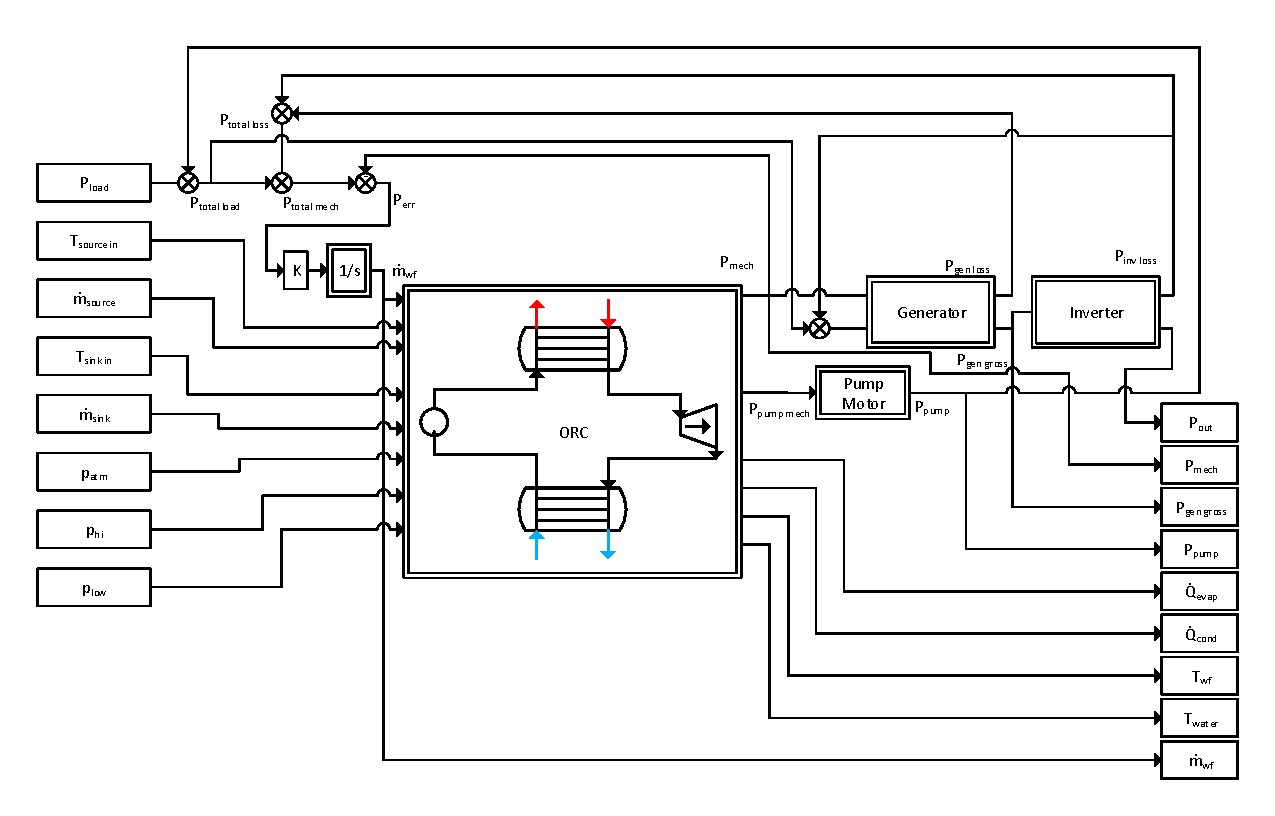
\includegraphics[width=\textwidth]{figures/Full Model Flow Diagram.pdf} 

	\caption{Organic Rankine cycle prime power system model diagram documenting data flows of the model. Boxes on the left side represent variable inputs, and those on the right indicate variable outputs.}
	\label{fig:full_flow_diagram_label}

\end{figure}


\cleardoublepage